\documentclass[11pt,a4paper]{article}

\usepackage[T1]{fontenc}
\usepackage[utf8]{inputenc}
\usepackage[ngerman]{babel}
\usepackage{lmodern}
\usepackage[a4paper,margin=2.5cm]{geometry}
\usepackage{microtype}
\usepackage{parskip}
\usepackage{csquotes}
\usepackage{enumitem}
\usepackage{graphicx}
\usepackage{tabularx}
\usepackage{wrapfig}
\usepackage[hidelinks]{hyperref}

\setlist[enumerate]{leftmargin=*,label=\arabic*.}

\title{Anfrage zur Filmvorf\"uhrung von \enquote{Die Kommissarin} in Karlshorst\\mit Gespr\"ach am 19.~April~2026}
\author{}
\date{}

\begin{document}

\maketitle
\vspace{-0.95cm}
\noindent
\begin{minipage}[t]{0.70\textwidth}
\footnotesize Hiermit m\"ochten wir anfragen, ob Karlshorst am 19.~April~2026 bereit w\"are, eine Filmvorf\"uhrung mit anschlie{\ss}endem Gespr\"ach auszurichten. Die Veranstaltung wird vom \href{https://eles-studienwerk.de/}{Ernst Ludwig Ehrlich Studienwerk (ELES)} im Rahmen der Abendveranstaltungsreihe \href{https://gemeinsam-gegen-antisemitismus.de/}{\enquote{Nie wieder!? Gemeinsam gegen Antisemitismus \& f\"ur eine plurale Gesellschaft}} organisiert. Sie richtet sich an die Stipendiat:innen des Ernst Ludwig Ehrlich Studienwerks sowie an die \"Offentlichkeit; die Veranstaltung ist als kostenfreies Angebot mit Voranmeldung angedacht.
\end{minipage}\hfill
\begin{minipage}[t]{0.25\textwidth}
\footnotesize
\vspace{-0.1cm}
\raggedleft
\href{https://gemeinsam-gegen-antisemitismus.de/}{
\includegraphics[width=\linewidth,height=4.4\baselineskip,keepaspectratio]{NW_Logo_quer2_inverted.png}}
\end{minipage}
\vspace{-0.2cm}

\section*{Der Film und sein historischer Kontext}

\begin{wrapfigure}[12]{r}{0.24\textwidth}
  \vspace{-1.1\baselineskip}
  \centering
  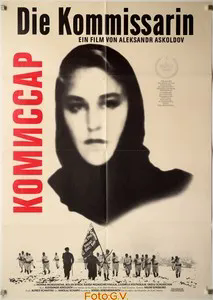
\includegraphics[width=\linewidth]{Kommissarin_plakat.png}
\end{wrapfigure}

Aleksandr Askoldovs Film \enquote{Die Kommissarin} entstand 1967 nach Wassili Grossmans Erz\"ahlung \enquote{In der Stadt Berdytschiw}. Berdytschiw erscheint darin als j\"udisch gepr\"agter Raum des ehemaligen Zarenreichs, in dem Revolution, B\"urgerkrieg und Alltag ineinandergreifen. Im Zentrum steht die schwangere Kommissarin Klawdija Wawilowa, die bei einer armen j\"udischen Familie unterkommt. So verschiebt der Film den Blick von der politischen Gro{\ss}geschichte auf N\"ahe, Verletzlichkeit und existenzielle Unsicherheit.

Askoldov zeigt Geschichte nicht heroisch, sondern als Raum von Gewalt, Abh\"angigkeit und moralischer Desorientierung. Historische Dramatik, Groteske und traumartige Bilder verdichten diese Erfahrung zu einer br\"uchigen, bedrohlichen Landschaft.

Zugleich r\"uckt der Film eine j\"udisch-sowjetische Erfahrungswelt ins Zentrum, die im sowjetischen Kino meist marginal blieb. Im Pogrom kulminieren B\"urgerkriegsgewalt, antisemitische Deutungsmuster wie der Mythos der sogenannten \enquote{\.Zydokomuna} (\enquote{Jewish Bolshevism}) und der sp\"atere Schatten der Shoah. Gerade deshalb wurde \enquote{Die Kommissarin} verboten und erst w\"ahrend der Glasnost \"offentlich gezeigt. Heute gilt der Film als Schl\"usselwerk, weil er die Verbindung von B\"urgerkrieg, Pogromgewalt und j\"udisch-sowjetischer Erinnerung sichtbar macht.

\section*{Kurzkonzeption}

Die Veranstaltung nimmt \enquote{Die Kommissarin} zum Ausgangspunkt f\"ur ein Gespr\"ach \"uber j\"udisch-sowjetische Erfahrung, Krieg und Erinnerung. Der Film geh\"ort nicht nur zur sowjetischen Filmgeschichte, sondern auch zu einer Geschichte von Zensur, Ausschluss und versp\"ateter Sichtbarkeit. Er zeigt eine j\"udisch-sowjetische Welt im historischen Umbruch, zwischen Revolution, B\"urgerkrieg, Gewalt und Bedrohung.

F\"ur Kino Kaddish ist der Film besonders geeignet, weil er j\"udisch-sowjetische Erfahrung, osteurop\"aische Gewaltgeschichte und Erinnerungspolitik zusammenf\"uhrt. Berditschew erscheint als Ort j\"udisch-sowjetischen Lebens; zugleich verweist der Film von den Pogromen der B\"urgerkriegszeit auf den sp\"ateren Horizont der Shoah. Sichtbar werden Alltag, Verletzlichkeit und prek\"are Zugeh\"origkeit dort, wo offizielle Geschichtsbilder diese Erfahrung lange an den Rand gedr\"angt haben.

Karlshorst bietet daf\"ur einen pr\"agnanten Rahmen: Hier kreuzen sich Erinnerungen an Kriegsende, Kapitulation und Befreiung mit der Frage, welche Geschichten sichtbar werden. Der Film setzt damit einen Gegenakzent zu einer vorwiegend milit\"arischen oder staatlichen Erz\"ahlung. Die Grundidee des Abends ist, \enquote{Die Kommissarin} als Zugang zu j\"udischer Identit\"at in der Sowjetzeit zu rahmen. Es sollen Erfahrungen j\"udischer Gemeinschaften hervortreten, die von diesem Hintergrund gepr\"agt sind. Zugleich soll eine geschichtliche \"Uberlieferung sichtbar werden, die einem westlichen Publikum oft wenig vertraut ist.

\section*{Gespr\"achspartnerinnen}

\textbf{\href{https://www.zfl-berlin.org/person/scherbakowa.html}{Prof.\ Dr.\ Irina Scherbakowa}} ist Germanistin, Historikerin und Mitbegr\"underin der Menschenrechtsorganisation \href{https://www.memorial.de/}{MEMORIAL}. Ihre Arbeit zu m\"undlicher Geschichte, Stalinismus und sowjetischer Erinnerungspolitik zeigt, wie der staatliche \enquote{Siegesmythos} unbequeme Erinnerungen systematisch verdr\"angte. F\"ur das Gespr\"ach bringt sie die Frage mit, warum ein Film wie \enquote{Die Kommissarin}, der j\"udische Verletzlichkeit statt revolution\"aren Heroismus zeigt, zwanzig Jahre lang unzeigbar war und was seine versp\"atete Sichtbarkeit \"uber sowjetische und postsowjetische Geschichtspolitik verr\"at.

\textbf{\href{https://www.dubnow.de/person/prof-dr-victoryia-a-sukovata}{Prof.\ Dr.\ Viktoriya Sukovata}} war an der Universit\"at Charkiw t\"atig und forscht derzeit als Gastwissenschaftlerin am Dubnow-Institut Leipzig. Ihre Arbeiten untersuchen, wie der Holocaust im sowjetischen und postsowjetischen Film dargestellt, verschl\"usselt oder unsichtbar gemacht wurde. Sie zeigt, dass j\"udisches Leid in der sowjetischen Kultur meist unter allgemeinen Kategorien wie \enquote{sowjetische Zivilisten} aufgel\"ost und antisemitische Gewalt selten eigens benannt wurde. Ihr Blick auf \enquote{Die Kommissarin} sch\"arft die Frage, was es bedeutet, dass Askoldov Berditschew als ausdr\"ucklich j\"udischen Raum inszeniert und die Pogromgewalt beim Namen nennt.

Gemeinsam er\"offnen beide Perspektiven einen Dialog \"uber die politischen und kulturellen Bedingungen, unter denen Erinnerung entsteht, unterdr\"uckt und wiedergewonnen wird.

\section*{Zeitplan}

\noindent\textbf{Sonntag, 19.~April~2026}

\small
\renewcommand{\arraystretch}{1.08}
\begin{tabularx}{\textwidth}{@{}p{3.1cm}X@{}}
\textbf{Zeit} & \textbf{Programmpunkt} \\
14:30--14:45 & \textbf{Ankommen und Begr\"u{\ss}ung}\\
& Treffpunkt vor dem Museum, kurze Einf\"uhrung. \\
14:45--16:00 & \textbf{Thematische F\"uhrung durch das Museum}\\
& Aufteilung in zwei Gruppen; Schwerpunkt: Karlshorst, Kapitulation, Vernichtungskrieg, j\"udisch-sowjetische Erinnerung. \\
16:00--16:20 & \textbf{Einf\"uhrung zum Film}\\
& Kurzer Vortrag zum historischen, literarischen und filmischen Kontext. \\
16:20--18:04 & \textbf{Filmvorf\"uhrung}\\
& Aleksandr Askoldovs \enquote{Die Kommissarin} (104 Min.). \\
18:04--19:00 & \textbf{Podiumsgespr\"ach mit Irina Scherbakowa und Viktoriya Sukovata (angefragt)}\\
& Diskussion \"uber Film, j\"udisch-sowjetische Erfahrung, Pogromgewalt, Shoah und Erinnerungskultur. \\
19:00--19:30 & \textbf{Offener Ausklang}\\
& Fragen, Austausch und Vernetzung. \\
\end{tabularx}

\end{document}
